\documentclass[11pt]{article}
\usepackage{amsmath, amssymb, amsthm}
\usepackage{geometry}
\usepackage{hyperref}
\usepackage{enumitem}
\usepackage{mathrsfs}
\usepackage{tikz}
\usetikzlibrary{arrows.meta}
\usepackage{float}
\geometry{margin=1in}
\title{Chapter 8 --- Vertex Colourings \\}
\author{Luca De Vecchis}
\date{Jan 2026}
\theoremstyle{definition}
\newtheorem{definition}{Definition}[section]
\newtheorem{theorem}{Theorem}[section]
\newtheorem{conjecture}{Conjecture}[section]
\newtheorem{remark}{Remark}[section]
\theoremstyle{plain}
\newtheorem{lemma}{Lemma}[section]
\usepackage{hyperref}
\hypersetup{
    colorlinks=true,
    linkcolor=blue,
    filecolor=magenta,      
    urlcolor=cyan,
}

\begin{document}

\maketitle
\tableofcontents
\newpage

\section{Chromatic Number}

\subsection{What is a vertex colouring?}
Let $G = (V, E)$ be a simple graph (no loops, no multiple edges). \\
A vertex colouring of $G$ is a function:
\[ c: V \to \{1, 2, \dots, k\} \]
such that:
\[ \text{if } uv \in E, \quad c(u) \neq c(v) \]

\paragraph{Interpretation}
\begin{itemize}
    \item Each vertex is assigned a colour (represented by an integer).
    \item Adjacent vertices must receive different colours.
    \item Non-adjacent vertices may share the same colour.
    \item This is a constraint satisfaction problem imposed by adjacency.
\end{itemize}

\subsection{Proper colourings and $k$-colourability}
A colouring that satisfies the adjacency condition is called a \textbf{proper colouring}.

\paragraph{Definition}
A graph $G$ is \textbf{$k$-colourable} if there exists a proper vertex colouring using at most $k$ colours.

\paragraph{Key points:}
\begin{itemize}
    \item ``At most'' is important.
    \item If a graph is $k$-colourable, it is also $(k+1)$-colourable, $(k+2)$-colourable, etc.
    \item The interesting question is the smallest such $k$.
\end{itemize}

\begin{figure}[h]
    \centering
    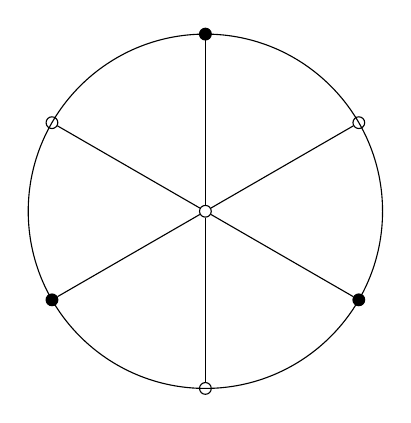
\begin{tikzpicture}[scale=1.5, every node/.style={circle, draw, inner sep=1.5pt}]
        % Central vertex
        \node (center) at (0,0) {};
        
        % Outer vertices - alternating filled/unfilled
        \foreach \a [count=\i] in {90, 150, 210, 270, 330, 30} {
            \ifodd\i
                \node[fill=black] (v\i) at (\a:1.5) {};
            \else
                \node[fill=white] (v\i) at (\a:1.5) {};
            \fi
            \draw (center) -- (v\i);
        }
        
        % Draw the outer circle
        \draw (0,0) circle (1.5);
    \end{tikzpicture}
    \caption{A 3-chromatic graph.}
    \label{fig:3-chromatic}
\end{figure}

\subsection{The chromatic number}
\paragraph{Definition (central concept)}
The chromatic number of a graph $G$, denoted $\chi(G)$, is the minimum number of colours required for a proper vertex colouring of $G$.
\[ \chi(G) = \min \{ k \mid G \text{ is } k\text{-colourable} \} \]
This number measures the intrinsic colouring complexity of the graph.

\subsubsection{First examples (essential intuition)}

\textbf{Empty graph $E$} \\
Let $E_n$ be a graph with $n$ vertices and no edges.
\begin{itemize}
    \item No adjacency constraints.
    \item All vertices may receive the same colour.
    \item $\chi(E_n) = 1 \quad (n \ge 1)$
\end{itemize}

\noindent \textbf{Complete graph $K_n$} \\
Every pair of vertices is adjacent.
\begin{itemize}
    \item Each vertex must have a different colour.
    \item $\chi(K_n) = n$
    \item This is the maximum possible chromatic number for a graph with $n$ vertices.
\end{itemize}

\noindent \textbf{Paths $P_n$} \\
A path alternates adjacency.
\begin{itemize}
    \item Colour vertices alternately (e.g., red–blue–red–blue).
    \item Works for any length.
    \item $\chi(P_n) = 2 \quad (n \ge 2)$
\end{itemize}

\noindent \textbf{Cycles $C_n$} \\
\begin{itemize}
    \item If $n$ is even: $\chi(C_n) = 2$
    \item If $n$ is odd: $\chi(C_n) = 3$
    \item The odd cycle is the smallest obstruction to 2-colourability.
\end{itemize}

\subsection{Bipartite graphs and 2-colourability}
\paragraph{Definition}
A graph is bipartite if its vertex set can be partitioned into two sets $V = A \cup B$ such that no edge joins two vertices in the same set.

\paragraph{Fundamental theorem}
A graph is bipartite if and only if $\chi(G) \le 2$. \\
Equivalently: A graph is 2-colourable $\iff$ It contains no odd cycle.

\subsection{Lower bounds for the chromatic number}
Determining $\chi(G)$ exactly is hard, so we study bounds.

\paragraph{Clique number}
A clique is a complete subgraph. Let $\omega(G) = \text{size of the largest clique in } G$. \\
Since all vertices in a clique are pairwise adjacent:
\[ \chi(G) \ge \omega(G) \]

\paragraph{Maximum degree}
Let $\Delta(G) = \max_{v \in V} \deg(v)$. \\
Trivially:
\[ \chi(G) \le \Delta(G) + 1 \]
(Reason: colour greedily.)

\subsection{The greedy colouring algorithm}
Order the vertices arbitrarily: $v_1, v_2, \dots, v_n$. Colour each vertex with the smallest available colour not used by its coloured neighbours.

\paragraph{Properties}
\begin{itemize}
    \item Uses at most $\Delta(G) + 1$ colours.
    \item Fast and simple but not optimal in general.
    \item Strongly dependent on vertex ordering.
\end{itemize}

\subsection{Chromatic number vs intuition}
\textbf{Important warning:} Sparse graphs can have large chromatic numbers. There exist graphs with no triangles, large girth, and arbitrarily large chromatic numbers. Chromatic number is not controlled by local density alone; global structure matters.

\subsection{Computational complexity}
Determining whether $\chi(G) \le k$ for a given $k \ge 3$ is \textbf{NP-complete}.
\begin{itemize}
    \item No known efficient algorithm.
    \item Exact computation is infeasible for large graphs.
\end{itemize}

\section{Brooks’ Theorem}

\subsection{Motivation: why Brooks’ Theorem matters}
From Section 8.1 we know:
\[ \chi(G) \le \Delta(G) + 1 \]
This bound is always true, but often far from tight. 

\paragraph{Natural question}
When do we actually need $\Delta(G) + 1$ colours? Brooks’ Theorem answers this almost completely.

\subsection{Statement of Brooks’ Theorem}
\textbf{Theorem (Brooks, 1941)} \\
Let $G$ be a connected graph. Then:
\[ \chi(G) \le \Delta(G) \]
unless $G$ is:
\begin{enumerate}
    \item A complete graph, or
    \item An odd cycle.
\end{enumerate}

\paragraph{Equivalently:}
\[ 
\chi(G) = 
\begin{cases} 
\Delta(G) + 1 & \text{if } G = K_n \text{ or } G = C_{2k+1}, \\
\le \Delta(G) & \text{otherwise.}
\end{cases} 
\]
This result is best possible.

\subsubsection{Understanding the exceptions}

\paragraph{Complete graphs}
For $K_n$:
\begin{itemize}
    \item $\Delta(K_n) = n - 1$
    \item $\chi(K_n) = n = \Delta + 1$
\end{itemize}
This is unavoidable because every vertex is adjacent to all others.

\paragraph{Odd cycles}
For $C_{2k+1}$:
\begin{itemize}
    \item $\Delta = 2$
    \item $\chi = 3 = \Delta + 1$
\end{itemize}
As seen earlier, odd cycles cannot be 2-coloured.

\paragraph{Key insight}
These are the only connected graphs that force the extra colour. Everything else can be coloured with at most $\Delta(G)$ colours.

\subsubsection{Why the theorem is surprising}
Intuitively, one might think high-degree vertices or local congestion force many colours. Brooks’ Theorem shows:
\begin{itemize}
    \item Degree alone \textit{almost} determines $\chi(G)$.
    \item Except for two very specific, rigid structures, $\Delta(G)$ is always enough.
\end{itemize}

\subsubsection{Examples to internalize the theorem}

\noindent \textbf{Even cycle $C_6$} \\
$\Delta = 2$. Not complete and not odd $\Rightarrow \chi(C_6) \le 2$. Indeed, $\chi(C_6) = 2$.

\noindent \textbf{A cubic graph (3-regular)} \\
Let $G$ be connected and every vertex has degree 3 ($\Delta = 3$). If $G \neq K_4$, then $\chi(G) \le 3$. Many nontrivial graphs (e.g., the Petersen graph) satisfy this.

\noindent \textbf{Trees} \\
For all trees except $K_1$, $\Delta \ge 1$. Since trees are bipartite, $\chi(G) = 2 \le \Delta$ (provided $\Delta \ge 2$; if $\Delta = 1$, the tree is $K_2$, which is an exception covered by the $K_n$ rule).

\subsubsection{Proof idea (high-level)}
The full proof is nontrivial and constructive. At an intuitive level:
\begin{itemize}
    \item Choose a vertex ordering that avoids conflicts.
    \item Exploit the absence of cliques or odd cycles.
    \item Use Kempe chains (recolouring arguments) to resolve bottlenecks.
    \item Force a greedy colouring to succeed with $\Delta$ colours.
\end{itemize}

\subsubsection{Why connectivity matters}
Brooks’ Theorem assumes connected graphs. If $G$ is disconnected, apply the theorem to each component and take the maximum $\chi(G)$ among them.

\subsubsection{Relation to earlier bounds}
Recall: $\omega(G) \le \chi(G) \le \Delta(G) + 1$. \\
Brooks refines this to:
\[ \omega(G) \le \chi(G) \le \Delta(G) \]
for all but two exceptional families. This is a dramatic tightening of the upper bound.

\subsubsection{Consequences and applications}
\begin{itemize}
    \item Shows that high chromatic number requires global structure.
    \item Motivates the study of critical graphs and the relationship between girth and chromatic number.
\end{itemize}

\subsubsection{Conceptual Interpretation}

Brooks' theorem characterizes graphs that are \emph{degree-critical} with respect to coloring. It plays a central role in the theory of critical graphs and serves as a foundational result in structural graph theory.

\subsection{Grötzsch Graph}

\paragraph{The Grötzsch Graph.}  
The Grötzsch graph is the smallest triangle-free planar graph with chromatic number 4. It has 11 vertices and 20 edges. Its importance lies in showing that **even planar graphs with no triangles can require four colors**, demonstrating that forbidding short cycles alone does not reduce the chromatic number below 4.

\begin{remark}
The Grötzsch graph connects directly to the theorem of the existence of triangle-free graphs with arbitrary chromatic number, providing a concrete, planar, minimal example for $k=4$. It is an extremal example in planar graph coloring, illustrating that girth constraints do not automatically lower $\chi(G)$ in planar graphs.
\end{remark}

\subsection{The Four-Color Theorem.}

\begin{theorem}[Four-Color Theorem]
Every planar graph can be properly colored with at most four colors, i.e., if $G$ is planar, $\chi(G) \le 4$.
\end{theorem}

\begin{remark}
- It implies that no planar graph requires more than four storage units in the planar storage analogy.  
- While the theorem sets a universal upper bound for planar graphs, the Grötzsch graph shows that even triangle-free planar graphs may achieve the maximum $\chi(G)=4$, so local sparsity is not sufficient to guarantee a 3-coloring.  
- Historically, this theorem was the first major result proven with extensive computer assistance (Appel and Haken, 1976), demonstrating both the complexity and subtlety of planar graph coloring.
\end{remark}

\paragraph{Connection to previous results:}
- Brooks' theorem: In planar graphs, $\Delta \le 5$, so Brooks’ theorem guarantees $\chi(G) \le \Delta(G)$ except for exceptional cases; the Four-Color Theorem provides a stronger global bound for planarity.  
- Chromatic polynomials: For planar graphs, $P_G(4) > 0$ always; Grötzsch graph shows $P_G(3) = 0$ even though the graph is triangle-free.  
- Girth vs. chromatic number: The Grötzsch graph is triangle-free ($girth \ge 4$) but still requires four colors.

\paragraph{Illustrative Example:}  
- Grötzsch graph (11 vertices) requires 4 colors; every proper 3-coloring attempt fails due to forced color conflicts, showing explicitly that $\chi(G)=4$ for a planar triangle-free graph.

\begin{figure}[H]
    \centering
    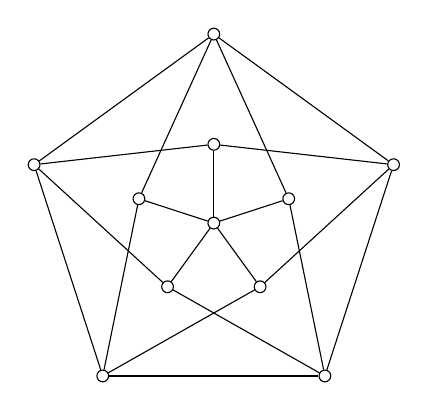
\begin{tikzpicture}[scale=2, every node/.style={circle, draw, inner sep=1.5pt, fill=white}]
        % Central vertex
        \node (center) at (0,0) {};
        
        % Inner 5-cycle (the star points)
        \foreach \i in {1,...,5} {
            \node (inner\i) at ({72*\i + 18}:0.5) {};
            \draw (center) -- (inner\i);
        }
        
        % Outer 5-cycle
        \foreach \i in {1,...,5} {
            \node (outer\i) at ({72*\i + 18}:1.2) {};
        }
        
        % Connections
        \foreach \i in {1,...,5} {
            \pgfmathtruncatemacro{\next}{mod(\i, 5) + 1}
            \draw (outer\i) -- (outer\next);
            
            \pgfmathtruncatemacro{\outA}{mod(\i+3, 5) + 1}
            \pgfmathtruncatemacro{\outB}{mod(\i, 5) + 1}
            \draw (inner\i) -- (outer\outA);
            \draw (inner\i) -- (outer\outB);
        }
    \end{tikzpicture}
    \caption{The Grötzsch graph—a 4-critical graph.}
    \label{fig:grotzsch}
\end{figure}


\section{Hajós’ Conjecture}
\subsection{Motivation: beyond Brooks’ Theorem}
From Brooks’ Theorem we learned that large degree alone does not force a large chromatic number. Only very rigid structures (cliques, odd cycles) force extremal behaviour.

\paragraph{Natural question}
If a graph has a large chromatic number, what must it look like? Hajós’ Conjecture is an attempt to answer exactly this by turning colouring theory into structural graph theory.

\subsection{Hajós’ Conjecture — informal idea}
Very loosely: Graphs with large chromatic number must contain ``highly connected'' structures resembling complete graphs.

\subsection{Precise statement of Hajós’ Conjecture}
\textbf{Conjecture (Hajós, 1940s)} \\
If a graph $G$ satisfies $\chi(G) \ge k$, then $G$ contains a \textbf{subdivision} of $K_k$.

\subsection{What does ``subdivision of $K_k$'' mean?}
This is the critical technical notion, also known as a \textbf{topological minor}.

\paragraph{Subdivision}
A subdivision of a graph $H$ is obtained by replacing edges of $H$ by paths, where these paths are internally vertex-disjoint.
\begin{itemize}
    \item Vertices of $H$ (branch vertices) remain.
    \item Edges may be ``stretched'' into paths.
\end{itemize}


\paragraph{Examples}
\begin{itemize}
    \item \textbf{Subdivision of $K_3$:} $K_3$ is a triangle. A subdivision replaces each edge with a path (e.g., a cycle $C_n$ for $n > 3$). It still ``looks like'' a triangle topologically.
    \item \textbf{Subdivision of $K_4$:} Contains four branch vertices where every pair is joined by internally disjoint paths.
\end{itemize}

\subsection{Why Hajós’ Conjecture is plausible}
\begin{itemize}
    \item $K_k$ itself has chromatic number $k$.
    \item Subdividing edges does not reduce the chromatic number (it usually maintains it or makes it harder to colour).
    \item High chromatic number suggests a dense interconnection, or a ``hidden $K_k$ inside.''
\end{itemize}

\subsubsection{Known results: what is true and what is false}

\paragraph{True for small $k$}
\begin{itemize}
    \item $k = 1, 2, 3$: Trivial.
    \item $k = 4$: True.
    \item $k = 5$: True (requires a non-trivial proof).
\end{itemize}

\paragraph{False in general}
For $k \ge 6$, \textbf{Hajós’ Conjecture is false}. There exist graphs with arbitrarily large chromatic numbers that contain no subdivision of $K_k$. This counter-intuitive result was a major surprise in the field.

\subsubsection{What replaces Hajós’ Conjecture?}
Although false, it inspired several deep results regarding the structure of graphs.

\paragraph{$k$-critical graphs}
A graph $G$ is \textbf{$k$-critical} if:
\begin{itemize}
    \item $\chi(G) = k$
    \item Removing any edge or vertex reduces the chromatic number.
\end{itemize}
These are the minimal obstructions to $(k-1)$-colourability.

\subsection{Connection to girth and extremal examples}
Erdős showed (probabilistically) that graphs can have \textbf{arbitrarily large girth} (no short cycles) and \textbf{arbitrarily large chromatic number}. These graphs have no large cliques, yet still require many colours, breaking naive intuition.

\subsubsection{Conceptual importance}
Hajós’ Conjecture framed the right questions, connecting colouring to topological structure and influencing:
\begin{itemize}
    \item Minors theory.
    \item Hadwiger’s Conjecture (a related, still open conjecture regarding graph minors).
    \item Modern structural graph theory.
\end{itemize}
\clearpage

\section{Chromatic Polynomials}

\subsection{Motivation: from ``how many colours?'' to ``how many colourings?''}
Up to now, we asked questions like: ``Can $G$ be coloured with $k$ colours?'' or ``What is $\chi(G)$?'' Now we ask: \textit{Given $k$ colours, how many proper colourings does $G$ have?} Surprisingly, the answer is always a polynomial in $k$.

\subsection{Definition of the chromatic polynomial}
\paragraph{Definition}
For a graph $G$, the chromatic polynomial $P_G(k)$ is defined as the number of proper vertex colourings of $G$ using $k$ colours.
\begin{itemize}
    \item $k$ is a variable (usually a positive integer).
    \item $P_G(k)$ counts proper colourings.
    \item Colours are labelled (red, blue, green, etc.).
\end{itemize}

\begin{figure}[H]
    \centering
    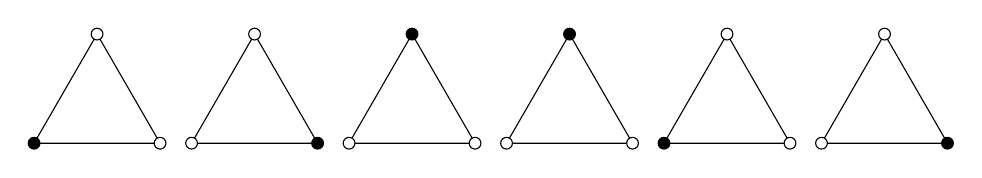
\begin{tikzpicture}[scale=0.8]
        % Define styles for the two types of vertices
        \tikzset{
            v_empty/.style={draw, circle, inner sep=1.5pt, fill=white},
            v_filled/.style={draw, circle, inner sep=1.5pt, fill=black}
        }

        % Triangle 1: Bottom-left filled
        \begin{scope}[shift={(0,0)}]
            \draw (0,0) node[v_filled] {} -- (2,0) node[v_empty] {} -- (1,1.732) node[v_empty] {} -- cycle;
        \end{scope}

        % Triangle 2: Bottom-right filled
        \begin{scope}[shift={(2.5,0)}]
            \draw (0,0) node[v_empty] {} -- (2,0) node[v_filled] {} -- (1,1.732) node[v_empty] {} -- cycle;
        \end{scope}

        % Triangle 3: Top filled
        \begin{scope}[shift={(5,0)}]
            \draw (0,0) node[v_empty] {} -- (2,0) node[v_empty] {} -- (1,1.732) node[v_filled] {} -- cycle;
        \end{scope}

        % Triangle 4: Top filled (same as 3)
        \begin{scope}[shift={(7.5,0)}]
            \draw (0,0) node[v_empty] {} -- (2,0) node[v_empty] {} -- (1,1.732) node[v_filled] {} -- cycle;
        \end{scope}

        % Triangle 5: Bottom-left filled
        \begin{scope}[shift={(10,0)}]
            \draw (0,0) node[v_filled] {} -- (2,0) node[v_empty] {} -- (1,1.732) node[v_empty] {} -- cycle;
        \end{scope}

        % Triangle 6: Bottom-right filled
        \begin{scope}[shift={(12.5,0)}]
            \draw (0,0) node[v_empty] {} -- (2,0) node[v_filled] {} -- (1,1.732) node[v_empty] {} -- cycle;
        \end{scope}

    \end{tikzpicture}
    \caption{Placeholder}
\end{figure}

A fundamental theorem due to Birkhoff and Whitney asserts that $P_G(k)$ is indeed a polynomial in $k$.

\subsection{Fundamental theorem}
\textbf{Theorem:} For every finite graph $G$, $P_G(k)$ is a polynomial in $k$ of degree $|V(G)|$.

\subsection{Immediate consequences}
\paragraph{Degree}
If $|V(G)| = n$, then $\deg P_G(k) = n$. The leading term is always $k^n$. 
\textit{Reason:} With no constraints (no edges), each vertex can be coloured independently in $k$ ways.

\paragraph{Integer coefficients with alternating signs}
The polynomial has the form:
\[ P_G(k) = k^n - a_1 k^{n-1} + a_2 k^{n-2} - \cdots \]
with $a_i \ge 0$. This reflects inclusion–exclusion over adjacency constraints.

\subsection{First concrete examples}

\noindent \textbf{Empty graph $E_n$} \\
No edges $\Rightarrow$ no constraints. $P_{E_n}(k) = k^n$.\\

\noindent \textbf{Complete graph $K_n$} \\
Every vertex must have a distinct colour.
\[ P_{K_n}(k) = k(k-1)(k-2)\cdots(k-n+1) \]
This is a falling factorial, often denoted $(k)_n$.\\

\noindent \textbf{Path $P_n$} \\
\begin{itemize}
    \item First vertex: $k$ choices.
    \item Each subsequent vertex: $k-1$ choices.
    \item $P_{P_n}(k) = k(k-1)^{n-1}$.\\
\end{itemize}

\noindent \textbf{Cycle $C_n$} \\
\[ P_{C_n}(k) = (k-1)^n + (-1)^n (k-1) \]
This formula explains why even cycles are 2-colourable and odd cycles are not.

\subsection{Deletion–contraction recurrence}
\noindent \textbf{Theorem (Deletion–Contraction)}
Let $e$ be an edge of $G$. Then:
\[ P_G(k) = P_{G - e}(k) - P_{G / e}(k) \]
Where:
\begin{itemize}
    \item $G - e$: graph with edge $e$ deleted.
    \item $G / e$: graph with edge $e$ contracted (endpoints merged).
\end{itemize}

\paragraph{Intuition}
$P_{G-e}(k)$ counts colourings ignoring the constraint at $e$, while $P_{G/e}(k)$ counts colourings where the endpoints of $e$ get the same colour. Subtracting the latter enforces the ``different colours'' rule.

\subsubsection{Example: $C_3 = K_3$}
Pick an edge $e$. 
\begin{itemize}
    \item $G - e = P_3$
    \item $G / e = K_2$
\end{itemize}
$P_{C_3}(k) = P_{P_3}(k) - P_{K_2}(k) = k(k-1)^2 - k(k-1) = k(k-1)(k-2)$.

\subsection{Chromatic number from the polynomial}
\[ \chi(G) = \min \{ k \in \mathbb{N} \mid P_G(k) > 0 \} \]
The polynomial encodes the chromatic number, but contains much more information about the graph's structure.

\subsection{Zeros and Importance}
\begin{itemize}
    \item Values where $P_G(k) = 0$ are \textbf{chromatic roots}. All non-negative integers less than $\chi(G)$ are roots.
    \item They connect graph theory to statistical physics (Potts model) and network reliability.
\end{itemize}



\section{Girth and Chromatic Number}

\subsection{The naïve intuition (that turns out to be wrong)}
From earlier sections, it is natural to believe that short cycles (especially triangles and odd cycles) force many colours, or that a large chromatic number must come from local density. One might assume that if a graph has no short cycles, it should be ``easy'' to colour. This intuition is false.\\

\noindent The girth of a graph $G$, denoted $g(G)$, is the length of the shortest cycle in $G$.
\begin{itemize}
    \item \textbf{Trees:} $g(G) = \infty$.
    \item \textbf{Triangle-free graphs:} $g(G) \ge 4$.
    \item \textbf{Bipartite graphs:} Contain no odd cycles, but may still have short even cycles (e.g., $C_4$).
\end{itemize}

\subsection{The central question}
How are girth and chromatic number related? Specifically:
\begin{itemize}
    \item Does large girth force a small chromatic number?
    \item Does a small chromatic number imply short cycles?
\end{itemize}
We know odd cycles force $\chi \ge 3$, but higher values of $\chi$ are more mysterious.

\subsection*{The shocking result (Erdős, 1959)}
\textbf{Theorem (Erdős)} \\
For every pair of integers $g \ge 3$ and $k \ge 2$, there exists a graph $G$ such that:
\[ g(G) \ge g \quad \text{and} \quad \chi(G) \ge k \]

\paragraph{Interpretation}
You can simultaneously have no short cycles (arbitrarily large girth) and a very large chromatic number. This shows that a large chromatic number does \textbf{not} require local density or short cycles; it destroys the ``local obstruction'' viewpoint.

\subsubsection{Why this is counter-intuitive}
Recall that bipartite graphs have no odd cycles and $\chi \le 2$. Odd cycles were the only obstruction to 2-colourability. One might expect higher chromatic numbers to require higher-order local structures, but Erdős proved that colouring difficulty can be globally distributed. No small local pattern explains it.

\subsubsection{Proof idea (The Probabilistic Method)}
The proof uses the probabilistic method, which was revolutionary in combinatorics.

\paragraph{High-level strategy}
\begin{enumerate}
    \item Start with a random graph on $n$ vertices.
    \item Show that, with positive probability, the graph has very few short cycles.
    \item Show that, with positive probability, it has a small \textbf{independence number} $\alpha(G)$.
    \item Remove one vertex from every short cycle.
\end{enumerate}

\paragraph{The Resulting Graph}
The final graph has a large girth (because we broke all short cycles) and a small maximum independent set. 

\paragraph{Key Insight}
Recall the relationship:
\[ \chi(G) \ge \frac{|V(G)|}{\alpha(G)} \]
By keeping $\alpha(G)$ very small relative to the number of vertices, we force the chromatic number to be arbitrarily large, even without any local cliques or triangles.

\subsection{The Mycielski Construction}

\subsubsection{Why Mycielski’s construction is important}
While Erdős’ theorem (Section 8.5) is probabilistic and non-constructive, the Mycielski construction is explicit, deterministic, and elementary. It provides concrete examples showing that one can increase the chromatic number without increasing the clique number, directly complementing Erdős’ results.

\subsubsection{The problem Mycielski addressed}
We know $\chi(G) \ge \omega(G)$ (cliques force colours). The question Mycielski answered was: \textit{Can we force a high chromatic number while keeping the clique number small?} His answer was a definitive yes, even for triangle-free graphs ($\omega = 2$).

\subsubsection{Definition}
Let $G = (V, E)$ be a graph with $V = \{v_1, v_2, \dots, v_n\}$. The Mycielskian $\mu(G)$ is constructed as follows:

\begin{enumerate}
    \item \textbf{Step 1: Duplicate vertices.} Create a new set $U = \{u_1, u_2, \dots, u_n\}$ where each $u_i$ corresponds to $v_i$.
    \item \textbf{Step 2: Copy adjacency.} For every edge $v_i v_j \in E$, add ``cross edges'' $u_i v_j$ and $u_j v_i$. (Note: no edges are added between $u_i$ and $u_j$).
    \item \textbf{Step 3: Add a new vertex.} Add a final vertex $w$ and connect it to every vertex in $U$.
\end{enumerate}

\paragraph{Summary of $\mu(G)$:}
\begin{itemize}
    \item $V(\mu(G)) = V \cup U \cup \{w\}$.
    \item Edges include the original edges in $V$, the cross edges between $U$ and $V$, and the star edges from $w$ to $U$.
\end{itemize}

\subsubsection{Key properties}
\noindent \textbf{Theorem 1:} $\chi(\mu(G)) = \chi(G) + 1$. \\
The vertex $w$ forces an extra colour, and a clever recolouring argument shows exactly one more is sufficient.\\

\noindent \textbf{Theorem 2:} $\omega(\mu(G)) = \omega(G)$. \\
In particular, if $G$ is triangle-free, $\mu(G)$ remains triangle-free.\\

\noindent \textbf{Theorem 3:} If $G$ has girth $\ge 4$, then $\mu(G)$ has girth $\ge 4$.

\subsubsection{Concrete example}
Start with the cycle $G = C_5$:
\begin{itemize}
    \item $\chi(C_5) = 3$ and it is triangle-free.
    \item $\mu(C_5)$ (the \textbf{Grötzsch graph}) has $\chi = 4$ and is still triangle-free.
    \item Applying it again, $\mu(\mu(C_5))$ has $\chi = 5$ and remains triangle-free.
\end{itemize}
This allows for the creation of an infinite family of triangle-free graphs with unbounded chromatic number.

\begin{figure}[H]
    \centering
    \begin{tikzpicture}[
        scale=1.2, 
        vnode/.style={draw, circle, inner sep=1.2pt, fill=white}, 
        >=Stealth]

        % --- TOP ROW: G2 to G3 ---
        % G2
        \begin{scope}[shift={(0,5)}]
            \node (v1) at (0,0) [vnode, label=above:$v_1$] {};
            \node (v2) at (3,0) [vnode, label=above:$v_2$] {};
            \draw (v1) -- (v2);
            \node[draw=none] at (1.5,-1) {$G_2$};
        \end{scope}

        % Arrow 1
        \draw[thick, ->] (3.5,5) -- (4.5,5);

        % G3 (Star shape construction)
        \begin{scope}[shift={(6,5)}]
            \node[vnode, label=above:$v$] (v) at (90:1.5) {};
            \node[vnode, label=left:$v_1$] (v1) at (162:1.5) {};
            \node[vnode, label=right:$v_2$] (v2) at (18:1.5) {};
            \node[vnode, label=below:$u_1$] (u1) at (234:1.5) {};
            \node[vnode, label=below:$u_2$] (u2) at (306:1.5) {};
            
            \draw (v1) -- (v2);
            \draw (v) -- (u1) -- (v2);
            \draw (v) -- (u2) -- (v1);
            \node[draw=none] at (0,-2) {$G_3$};
        \end{scope}

        % --- BOTTOM ROW: G3 to G4 ---
        % G3 (Pentagon)
        \begin{scope}[shift={(0,0)}]
            \foreach \a [count=\i] in {90, 18, 306, 234, 162}
                \node[vnode, label=\a:$v_{\i}$] (v\i) at (\a:1.5) {};
            \draw (v1) -- (v2) -- (v3) -- (v4) -- (v5) -- (v1);
            \node[draw=none] at (0,-2) {$G_3$};
        \end{scope}

        % Arrow 2
        \draw[thick, ->] (2.5,0) -- (3.5,0);

        % G4 (Mycielskian of G3)
        \begin{scope}[shift={(6,0)}]
            % Outer vertices v
            \foreach \a [count=\i] in {90, 18, 306, 234, 162}
                \node[vnode, label=\a:$v_{\i}$] (v\i) at (\a:2) {};
            % Inner vertices u
            \foreach \a [count=\i] in {90, 18, 306, 234, 162}
                \node[vnode, label=\a:$u_{\i}$] (u\i) at (\a:1) {};
            % Center vertex v
            \node[vnode, label=above right:$v$] (vcenter) at (0,0) {};

            % Draw outer pentagon
            \draw (v1) -- (v2) -- (v3) -- (v4) -- (v5) -- (v1);
            % Draw connections to center
            \foreach \i in {1,...,5} \draw (u\i) -- (vcenter);
            % Draw Mycielskian edges (u_i to neighbors of v_i)
            \draw (u1) -- (v2) (u1) -- (v5);
            \draw (u2) -- (v1) (u2) -- (v3);
            \draw (u3) -- (v2) (u3) -- (v4);
            \draw (u4) -- (v3) (u4) -- (v5);
            \draw (u5) -- (v4) (u5) -- (v1);
            
            \node[draw=none] at (0,-2.5) {$G_4$};
        \end{scope}

    \end{tikzpicture}
    \caption{Mycielski's Construction}
\end{figure}

\subsubsection{Conceptual meaning}
The Mycielski construction shows that colouring difficulty can be forced globally in a controlled way. It provides a constructive counterweight to Erdős’ probabilistic method and explains why local density (cliques) is not the sole driver of the chromatic number.

\subsubsection*{7. Relationship to Hajós’ Conjecture}
Mycielski graphs are useful counter-examples in colouring theory because they possess a high chromatic number without containing large complete subgraphs, illustrating why conjectures like Hajós’ (which look for $K_k$ subdivisions) become so difficult to satisfy as $k$ increases.
\clearpage

\section{A Storage Problem}

\subsection{The real-world problem (informal statement)}
Consider a collection of items (chemicals, data blocks, or tasks) where certain pairs cannot be stored together due to interference, incompatibility, or resource conflicts. The goal is to:
\begin{itemize}
    \item Store all items using the \textbf{minimum number of storage units}.
    \item Ensure no incompatible items share the same unit.
\end{itemize}
This is a classic optimization problem.

\subsection{Graph-theoretic modelling}
We translate this real-world scenario into the language of graph theory:

\paragraph{Step 1: Construct the graph}
Define a graph $G = (V, E)$ as follows:
\begin{itemize}
    \item \textbf{Vertices ($V$):} Each item corresponds to a vertex.
    \item \textbf{Edges ($E$):} An edge $uv$ exists if items $u$ and $v$ are incompatible.
\end{itemize}
This is known as a \textbf{conflict graph}.

\paragraph{Step 2: Interpret storage units as colours}
\begin{itemize}
    \item Assign a colour to each vertex.
    \item Vertices of the same colour represent items stored together in the same unit.
    \item Adjacent vertices must have different colours to avoid conflicts.
\end{itemize}
This is exactly a \textbf{proper vertex colouring}.

\subsection{Core equivalence}
The minimum number of storage units required is the \textbf{chromatic number} $\chi(G)$ of the conflict graph.

\paragraph{Why this formulation is powerful}
Once modelled, all results from Sections 8.1–8.5 apply:
\begin{itemize}
    \item \textbf{Brooks’ Theorem:} Provides degree-based bounds for storage units.
    \item \textbf{Chromatic Polynomials:} Allows us to count the number of ways to assign items to $k$ units.
    \item \textbf{Girth/Mycielski:} Warns us that global complexity can remain high even if items only conflict with a few neighbors.
\end{itemize}

\paragraph{Example: Chemical Storage}
Suppose 5 chemicals have incompatibilities forming a cycle $C_5$.
\begin{itemize}
    \item Maximum degree $\Delta = 2$.
    \item However, $\chi(C_5) = 3$.
\end{itemize}
\textbf{Conclusion:} Even though each chemical conflicts with only two others, three storage units are unavoidable. This mirrors Brooks’ Theorem (odd cycles).

\subsection{Why greedy strategies may fail}
A naïve ``first-available-spot'' strategy is essentially a \textbf{greedy colouring}. 
\begin{itemize}
    \item \textbf{Problem:} Depending on the order of items, the algorithm may use more than $\chi(G)$ units.
    \item This reflects the \textbf{NP-hardness} of finding an optimal storage solution for large, complex conflict graphs.
\end{itemize}

\subsection{Interpretation using independent sets}
Each storage unit represents an \textbf{independent set} in $G$. The storage problem is fundamentally a task of partitioning $V(G)$ into the minimum number of independent sets. This connects graph colouring to:
\begin{itemize}
    \item Scheduling (tasks using the same resource).
    \item Channel assignment in telecommunications.
    \item Register allocation in compiler design.
\end{itemize}



\end{document}